%%%%%%%%%%%%%%%%%%%%%%%%%%%%%%%%%%%%%%%%%%%%%%%%%%%%%%%%%%%%%%%%%%%%%%%%%%%%%%%
%                         File: osa-revtex4-1.tex                             %
%                        Date: April 15, 2013                                 %
%                                                                             %
%                              BETA VERSION!                                  %
%                   JOSA A, JOSA B, Applied Optics, Optics Letters            %
%                                                                             %
%            This file requires the substyle file osajnl4-1.rtx,              %
%                   running under REVTeX 4.1 and LaTeX 2e                     %
%                                                                             %
%                   USE THE FOLLOWING REVTeX 4-1 OPTIONS:                     %
% \documentclass[osajnl,twocolumn,showpacs,superscriptaddress,10pt]{revtex4-1}%
%                    %% Use 11pt for Applied Optics                           %
%                                                                             %
%               (c) 2013 The Optical Society of America                       %
%                                                                             %
%%%%%%%%%%%%%%%%%%%%%%%%%%%%%%%%%%%%%%%%%%%%%%%%%%%%%%%%%%%%%%%%%%%%%%%%%%%%%%%

\documentclass[osajnl,twocolumn,showpacs,superscriptaddress,10pt]{revtex4-1} %% use 11pt for Applied Optics
%\documentclass[osajnl,preprint,showpacs,superscriptaddress,11pt]{revtex4-1} %% use 12pt for preprint option
\usepackage{amsmath,nccmath,amssymb,graphicx,float,minted,xparse,tikz}
\usepackage[utf8]{inputenc}
\graphicspath{{images/}}

\usepackage{mathtools,enumitem}
\usepackage{minted}

\begin{document}

\title{Programación Distribuida y Tiempo Real}

\author{Ulises Jeremias Cornejo Fandos}
\affiliation{Licenciatura en Informática, Facultad de Informática, UNLP}

\maketitle %% required

\section{Identifique similitudes y diferencias entre los sockets en C y en Java}

Para la creación y utilización de sockets en C se utiliza la librería estandar \textit{sys/socket.h}, mientras que en Java se utiliza la librería \textit{java.net} para la creación de los mismos y algunos módulos provenientes de la librería \textit{java.io} para interactuar con los mismos a modo de lectura y escritura. \\

Una diferencia muy marcada es el enfoque de implementación de los Sockets en ambos lenguajes. Por un lado tenemos el enfoque de Java, que cuenta con una clase \textit{java.net.Socket}. La misma permite establecer una comunicación bidireccional entre dos procesos en una red dada (el programa que define el socket y otro en la red). Además, se cuenta con la clase \textit{java.net.ServerSocket} para definir más directamente sockets que estén escuchando y aceptando conexiones desde procesos clientes. \\

Por otro lado, en C no se encuentra tal distinción. El modelo Cliente/Servidor puede ser implementado pero la librería no cuenta con funciones pensadas explicitamente para la realización de esta tarea. La librería \textit{sys/socket.h} expone la función \textbf{\textit{socket}} la cual permite crear un socket. \\

En C, todos los sockets son representados por file descriptors, de los cuales solo se conoce un número de identificación. Estos son utilizados de la misma manera que archivos de un file system, leyendo y escribiendo en ellos con las mismas operaciones. Adicionalmente se utilizan las operaciones \textit{bind}, \textit{listen} y \textit{accept} sobre el socket servidor para darle una dirección, permitirle escuchar por conexiones y aceptarlas respectivamente.

\section{Tanto en C como en Java (directorios csock-javasock):}

\subsection{¿Por qué puede decirse que los ejemplos no son representativos del modelo c/s?}

En el modelo cliente/servidor (c/s), el servidor está  la espera continua de algún pedido de conexión por parte de algún cliente. Luego, el esquema general de trabajo en un modelo c/s dado el pedido de conexión es el siguiente: inicialización (o handshape), transferencia de datos, y finalización.

En este caso, el servidor cierra la conexión dada la primer request y envio de respuesta. No se respetan los pasos de conexión anteriormente mencionados, pues en el ejemplo solo se realiza la transferencia de datos, sin envio de handshape o envío de mensajes de cierre de conexión.

\subsection{Muestre que no necesariamente siempre se leen/escriben todos los datos involucrados en las comunicaciones con una llamada read/write con sockets. Sugerencia: puede modificar los programas (C o Java o ambos) para que la cantidad de datos que se comunican sea de $10^3$ , $10^4$ , $10^5$ y $10^6$ bytes y contengan bytes asignados directamente en el programa (pueden no leer de teclado ni mostrar en pantalla cada uno de los datos del buffer), explicando el resultado en cada caso. Importante: notar el uso de “attempts” en “...attempts to read up to count bytes from file descriptor fd...” así como el valor de retorno de la función read (del man read).}

Se modificó la implementación del cliente y servidor de forma tal que el tamaño del buffer pueda ser definido en tiempo de compilación. (\textit{Ver implementación en la sección \ref{apendix:2b}}). \\

El tamaño del buffer tanto del cliente como del servidor se fue modificando con diferentes valores para ver hasta qué cantidad de datos podía leer, se probó con los siguientes valores: $10^3$ , $10^4$ , $10^5$ y $10^6$. \\

El servidor pudo leer correctamente todos los caracteres para un buffer size menor o igual a $10^4$. Sin embargo, cuando se probó con un buffer size de $10^5$, solo pudo leer $\approx 65480$ caracteres.

\subsection{Agregue a la modificación anterior una verificación de llegada correcta de los datos que se envían (cantidad y contenido del buffer), de forma tal que se asegure que todos los datos enviados llegan correctamente, independientemente de la cantidad de datos involucrados.}

Para realiza esta implementación see agregó en el cliente y servidor una función de hashing, \mintinline{c}{unsigned long djb2(unsigned char *str);}, la cual genera un hash de los datos recibidos para después utilizarlo al realizar un checksum. (\textit{Ver implementación en la sección \ref{apendix:2c}}).

El cliente genera un hash de los datos que se van a enviar. Una vez generado, se envían los datos, y se espera la respuesta del servidor para saber si los mismos fueron recibidos. Luego se envía el hash de los datos y el tamaño de los datos enviados. (\textit{Ver \ref{apendix:2c_client}}).

Por otra parte, el servidor espera los datos, el hash y el tamaño de los datos enviados por el cliente. Una vez que tiene todo esto, genera el hash de los datos recibidos y compara el hash y la cantidad de datos recibidos con el hash que se recibió y el tamaño de los datos que envia el cliente. (\textit{Ver \ref{apendix:2c_server}}).

\subsection{Grafique el promedio y la desviación estándar de los tiempos de comunicaciones de cada comunicación. Explique el experimento realizado para calcular el tiempo de comunicaciones.}

Para medir los tiempos de ejecución se utiliza la función \textit{dwalltime} para medir el tiempo existente entre el comienzo de la transmisión de datos y la confirmación del servidor de los mismos fueron recibidos. (\textit{Ver implementación en la sección \ref{apendix:2d}}).

Para la realización de los experimentos se miden los tiempos de transmisión de $10^3$, $10^4$, $10^5$ y $10^6$ bytes. Cada una de estas configuraciones se ejecutan 10 veces.

Luego, los tiempos recolectados en las pruebas se utilizan para calcular la media y desviación estándar para el envío de cada cantidad de datos.

\begin{figure}[H]
    \centering
    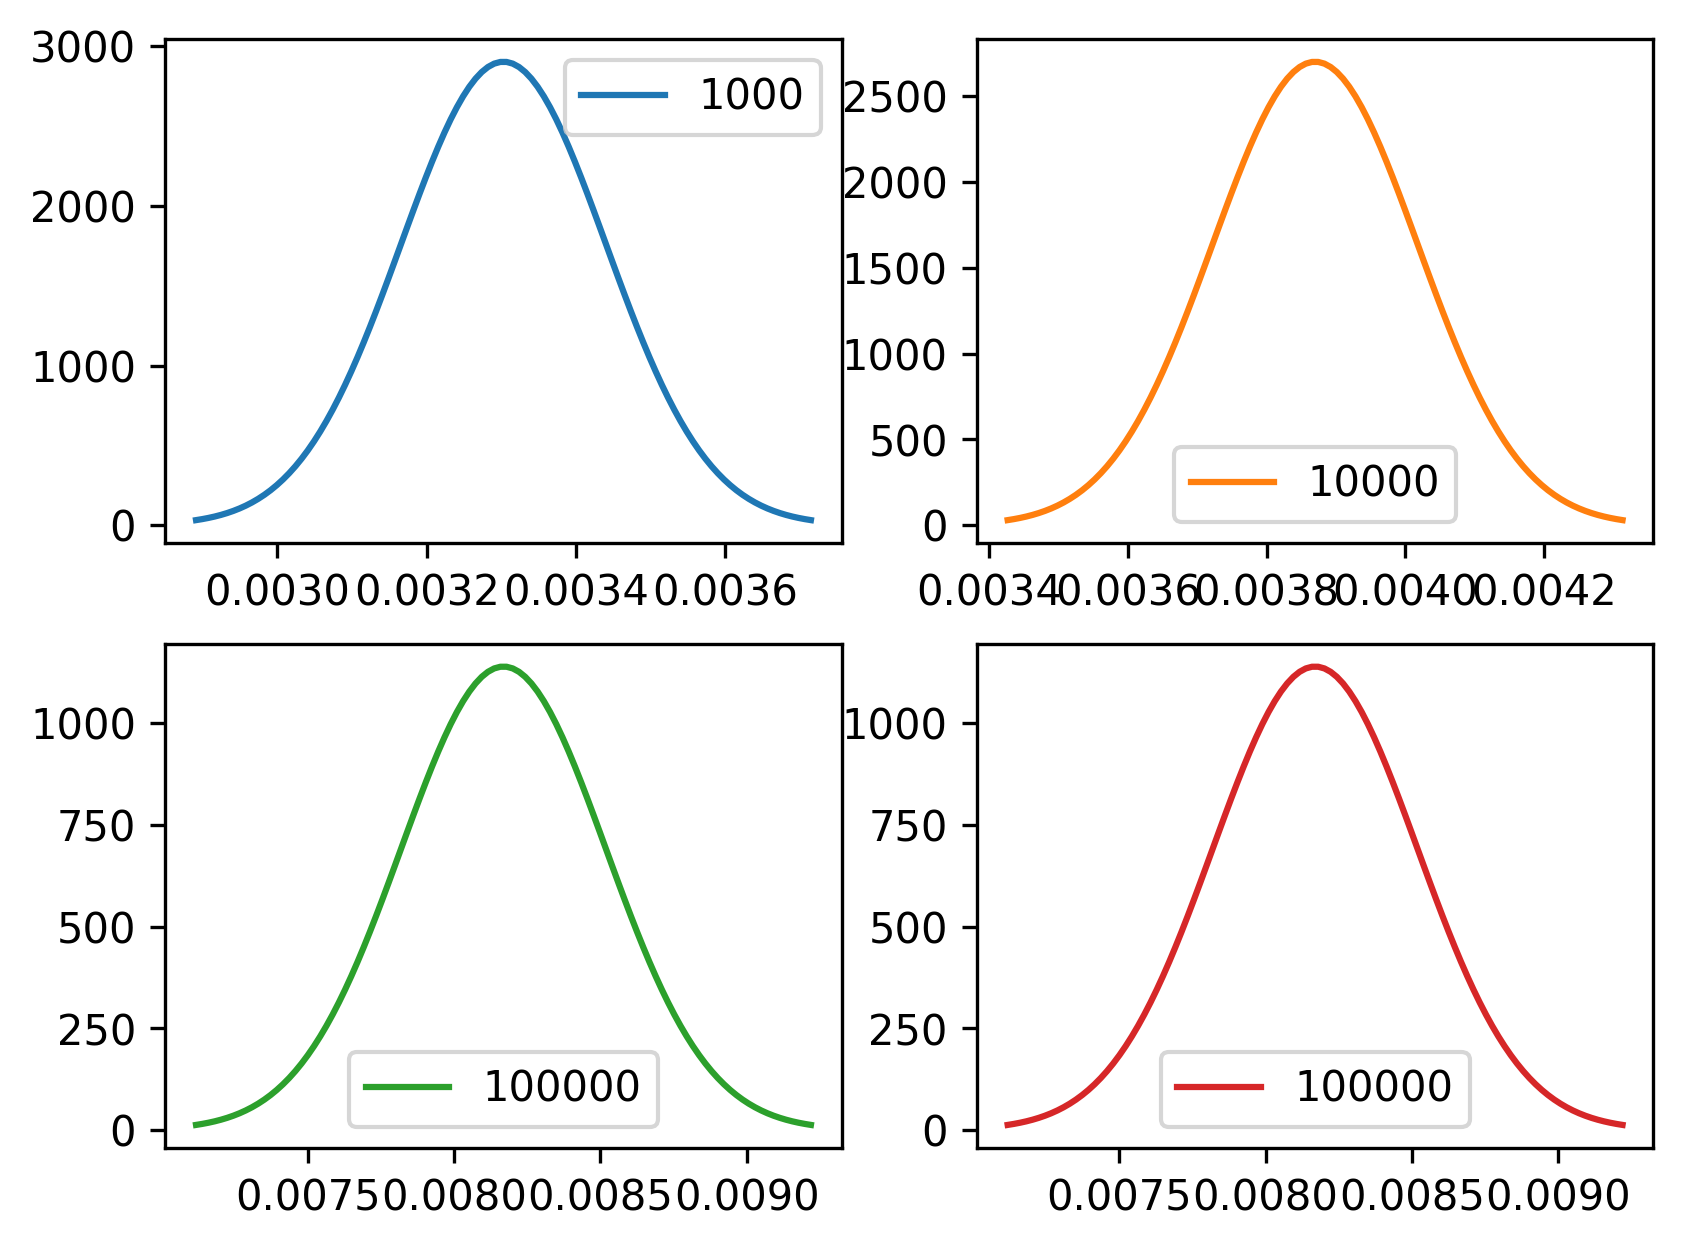
\includegraphics[width=0.45\textwidth]{graph_multi}
    \caption{Gráficas de las curvas gaussianas para cada escenario utilizando buffer size de $10^3$, $10^4$, $10^5$ y $10^6$.}
    \label{figure:summary_flatten}
\end{figure}

\begin{figure}[H]
    \centering
    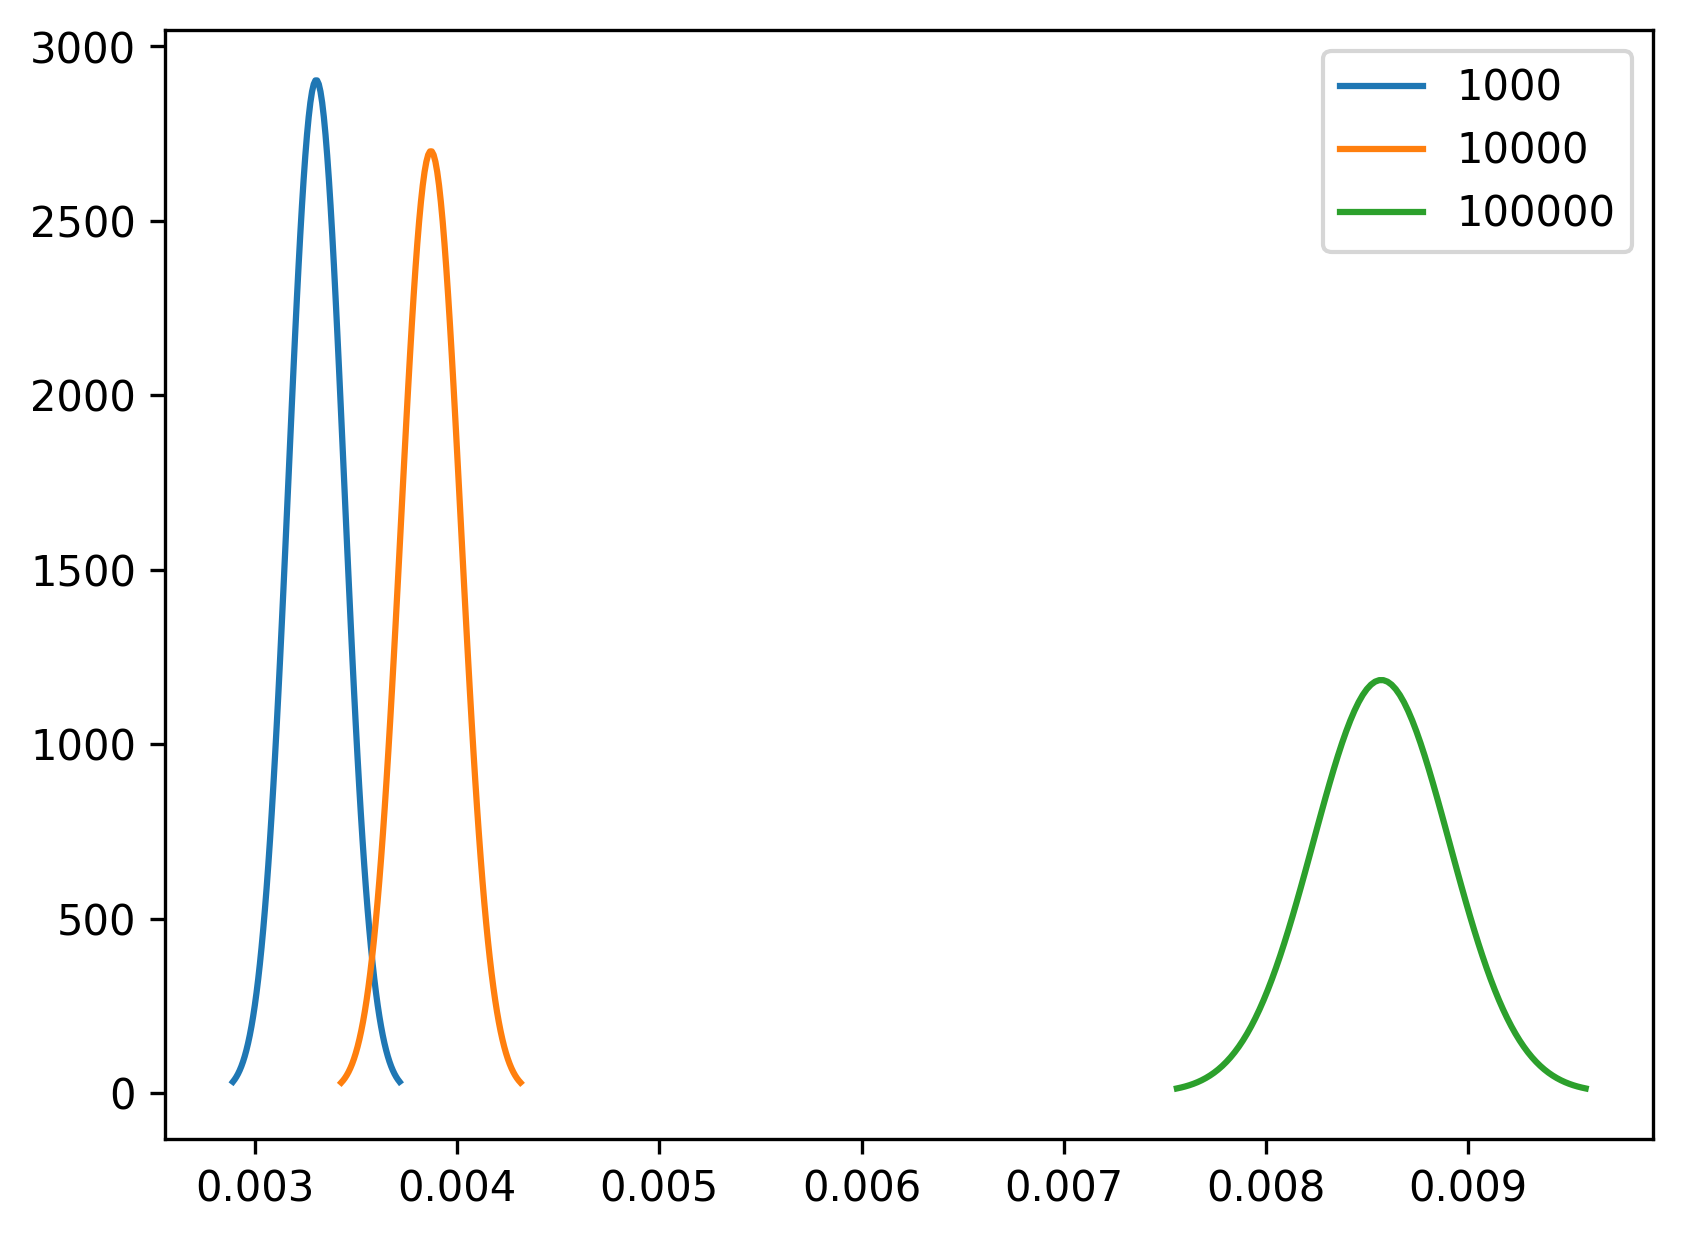
\includegraphics[width=0.45\textwidth]{graph}
    \caption{Gráfica comparativa de las curvas gaussianas para cada escenario utilizando buffer size de $10^3$, $10^4$ y $10^5$.}
    \label{figure:summary}
\end{figure}

\section{¿Por qué en C se puede usar la misma variable tanto para leer de teclado como para enviar por un socket? ¿Esto sería relevante para las aplicaciones c/s?}

El header o prototipo de la función \textit{write} en C está dado por la siguiente expresión:

\begin{minted}{c}
size_t write(int fd, void *buf, size_t nbytes);
\end{minted}

donde \textit{buf} es un puntero al espacio de memoria de \textit{nbytes} bytes a partir del cual la system call obtendrá la información para escribir en el file descriptor. \\

Luego, el valor enviado como segundo argumento de la función \textit{write} será cualquier puntero a un espacio de memoria, sea dinámica o estática. Es decir, podría enviar una referencia a un espacio de enteros (\mintinline{c}{int *}), espacio de caracteres (\mintinline{c}{char *}), etc.

En el caso de la variable utilizada para leer de teclado, la misma se define como sigue: \mintinline{c}{char buffer[256];}

Por lo tanto, buffer es una variable de tipo puntero, la cual referencia un espacio de memoria de caracteres alocado en forma estática.

Es por esto que, dado que \textit{write} espera un argumento de tipo puntero y la variable \textit{buffer} tiene ese tipo, puedo utilizar la misma variable tanto para entrada de texto del teclado como para el envio del mismo por un socket. \\

Esta potencia al momento de manejar memoria y punteros tiene ciertas desventajas al momento de programar una arquitectura como el modelo c/s. Se deben contar con precauciones dado que, siendo siempre un espacio de bytes, dependerá de como el cliente interprete los datos presentes en el espacio de memoria recibido al momento de acceder a la información.

\section{¿Podría implementar un servidor de archivos remotos utilizando sockets? Describa brevemente la interfaz y los detalles que considere más importantes del diseño. No es necesario implementar.}

Para plantear una implementación de servidor de archivos remotos utilizando sockets puedo basar mi solución en dos protocolos existente que definen una interfaz para este tipo de implementaciones, \textbf{FTP} y \textbf{TFTP}.

\begin{itemize}
    \item \textbf{FTP}
    
    Una implementación de FTP puede realizarse utilizando dos sockets de tipo TCP para el servidor. Los mismos pueden escuchar en los puertos estandar, 20 y 21, para datos y control respectivamente.
    
    Se cuenta con funciones específicas, entre otras las cuales se ejecuten sobre el \textit{filesystem} del servidor remoto FTP.
    
    \item \textbf{TFTP}
    
    Por otro lado, una implementación de TFTP se implementa como un servidor que utiliza unicamente un socket de tipo UDP. El conjunto de instrucciones soportadas por el mismo serán menores a las soportadas por un servidor FTP.
\end{itemize}

Para la implementación propia de un servidor de archivos remotos opto por una alternativa similar a la que se plantea sobre un servidor FTP. Para realizar un servidor de este estilo se debe implementar una conexión TCP, es decir, un inicio y cierre de conexión de 3 vías o \textit{3-ways-handshape}. \\

\textit{Las instrucciones soportadas por el servidor implementado podrían ser las siguiente:}

\begin{itemize}
    \item \textbf{ls}
    
    Crea una lista de todos los archivos que se encuentran en el directorio actual.
    
    El cliente envía el comando \textit{ls} y luego, el servidor contesta con la lista de archivos que posee. Se debe verificar el tamaño de los datos enviados desde el servidor para asegurarse que lleguen todos.

    
    \item \textbf{pwd}
    
    Muestra el path absoluto del directorio actual.
    
    El cliente envia el comando \textit{pwd} y el servidor responde con el path absoluto del duirectorio actual de trabajo.
    
    \item \textbf{cd}
    
    El comando significa change directory (cambiar el directorio) y se usa para pasar a un directorio diferente. El comando \textbf{cd} sin argumentos se utiliza para tener acceso al directorio principal.
    
    El cliente envia el comando \textit{cd} con o sin argumentos y el servidor actualiza internamente el directorio de trabajo.
    
    \item \textbf{mkdir}
    
    El comando mkdir se utiliza para crear un directorio dentro del directorio actual. El uso de este comando se reserva para los usuarios que tengan acceso permitido.

    \item \textbf{get}
    
    Este comando permite recuperar un archivo que se encuentra en el servidor.
    
    El cliente envia el comando \textit{get}. Si el comando aparece seguido del nombre de un archivo, el archivo remoto se transfiere a la máquina local, dentro del directorio local actual. Si aparece seguido de dos nombres de archivos, el archivo remoto (el primer nombre) se transfiere a la máquina local en el directorio local actual con el nombre del archivo especificado (el segundo nombre). Si el nombre del archivo contiene espacios, será necesario introducido entre comillas.
    
    El servidor comprueba la existencia del archivo. Dada su existencia, se abre el archivo y comprueba su tamaño. Luego, genera un \textit{checksum} del archivo. Por último, envía el archivo y el \textit{checksum} por el socket para comprar si se recibió correctamente.
    
    \item \textbf{put}
    
    Este comando se utiliza para enviar un archivo local al servidor.
    
    Si el comando aparece seguido del nombre de un archivo, el archivo local se transfiere al servidor en el directorio remoto actual. Si el comando aparece seguido de dos nombres de archivos, el archivo local (el primer nombre) se transfiere al servidor en el directorio remoto actual, con el nombre del archivo especificado (el segundo nombre). Si el nombre del archivo contiene espacios, será necesario introducido entre comillas.
    
    Finalmente, con el objetivo de verificar que el archivo sea enviado correctamente, se comprueba el tamaño del archivo y se lo envía al servidor. Para realizar la comprobación, se envía un \textit{checksum}, el cual el servidor debe contrastar contra un \textit{checksum} del archivo que le llegó.

    \item \textbf{delete}
    
    Borra el archivo especificado en el servidor remoto.
    
    El cliente envía el comando \textit{delete} seguido del nombre del archivo que desea eliminar. El servidor comprueba la existencia del archivo, y lo elimina.
\end{itemize}

\section{Defina qué es un servidor con estado (stateful server) y qué es un servidor sin estado (stateless server).}

\begin{itemize}
    \item \textbf{Stateful Server}
    
    Un servidor con estado es aquel que mantiene el estado de la información del usuario en forma de sesiones. Este tipo de servidores recuerda los datos del cliente (estado) de una solicitud a la siguiente. Servidores con estado, almacenar estado de sesión. Por lo tanto, pueden realizar un seguimiento de qué clientes han abierto qué archivos, punteros de lectura y escritura actuales para archivos, qué archivos han sido bloqueados por qué clientes, etc.
    
    \item \textbf{Stateless Server}
    
    A diferencia de un servidor con estado, el servidor sin estado es aquel que no mantiene ningún estado de la información para el usuario. En este tipo de servidores, cada consulta es completamente independiente a la anterior. \\
    Sin embargo, los servidores sin estado pueden identificar al usuario si la solicitud al servicio incluye una identificación de usuario única que se asignó anteriormente al mismo. Ese identificador (ID) del usuario deberá pasarse en cada consulta, a diferencia del caso de los servidores con estado que mantienen este ID de usuario en la sesión y los datos de la solicitud no necesariamente deben contener este ID.
\end{itemize}

\clearpage

\onecolumngrid

\section{Apéndice}

\subsection{Ejercicio 2b} \label{apendix:2b}

Modificación de los programas en C que permite variar el tamaño de los buffers en tiempo de compilación.

\subsubsection{Cliente} \label{apendix:2b_client}

\inputminted[mathescape]{c}{../resources/csock/client_2b.c}

\subsubsection{Servidor} \label{apendix:2b_server}

\inputminted[mathescape]{c}{../resources/csock/server_2b.c}

\subsection{Ejercicio 2c} \label{apendix:2c}

Modificación de los programas en C que permita verificar la llegada correcta de los datos.

\subsubsection{Cliente} \label{apendix:2c_client}

\inputminted[mathescape]{c}{../resources/csock/client_2c.c}

\subsubsection{Servidor} \label{apendix:2c_server}

\inputminted[mathescape]{c}{../resources/csock/server_2c.c}

\subsection{Ejercicio 2d} \label{apendix:2d}

Modificación de los programas en C que permita verificar medir tiempo de conexión.

\subsubsection{Cliente} \label{apendix:2d_client}

\inputminted[mathescape]{c}{../resources/csock/client_2d.c}

\subsubsection{Servidor} \label{apendix:2d_server}

La implementación del servidor no se modificó respecto de la presente en la sección \ref{apendix:2c_server}.
\end{document}
